\section{FlashAttention: IO感知的高效注意力}
\label{sec:flash_attention}

第~\ref{sec:background}节介绍的Roofline模型揭示了一个关键洞察:现代GPU的算力远超内存带宽,决定性能的往往不是"能算多快",而是"数据能多快送达"。标准注意力机制正是这一瓶颈的典型案例——它需要将$O(N^2)$规模的中间结果反复写入显存,而这些IO操作成为真正的性能杀手。

FlashAttention的核心思想是重新组织计算顺序,使注意力矩阵\textbf{永远不离开GPU的高速缓存}。这不是数学上的近似,而是精确等价的重新排列——我们用更多的计算换取更少的内存访问,而现代GPU恰好计算过剩、带宽稀缺。

\subsection{动机:GPU内存层次结构}

\subsubsection{内存瓶颈分析}

现代GPU的计算能力远超内存带宽。以NVIDIA A100为例:
\begin{itemize}
    \item \textbf{计算能力}:312 TFLOPS(FP16 Tensor Core)
    \item \textbf{HBM带宽}:2 TB/s
    \item \textbf{SRAM容量}:20 MB(共享内存 + L1缓存)
    \item \textbf{SRAM带宽}:约19 TB/s
\end{itemize}

\textbf{算术强度}(Arithmetic Intensity)定义为每字节内存访问的FLOPs:
\begin{equation}
    \text{算术强度} = \frac{\text{FLOPs}}{\text{内存访问字节数}}
\end{equation}

对于A100,达到峰值计算需要算术强度 $\geq 156$ FLOPs/Byte。标准注意力的算术强度远低于此,因此是\textbf{内存受限}(Memory-Bound)的。

\subsubsection{标准注意力的IO问题}

标准注意力实现需要多次HBM读写:
\begin{enumerate}
    \item 从HBM读取$Q, K$,计算$S = QK^\top$,写回HBM
    \item 从HBM读取$S$,计算$P = \softmax(S)$,写回HBM
    \item 从HBM读取$P, V$,计算$O = PV$,写回HBM
\end{enumerate}

总HBM访问量:$O(N^2 + Nd)$,其中$N$是序列长度,$d$是头维度。对于长序列,$N^2$项主导,造成严重的IO瓶颈。

\subsection{FlashAttention v1}

FlashAttention~\citep{dao2022flashattention}的核心思想是:\textbf{永远不将完整的$N \times N$注意力矩阵写入HBM}。

\subsubsection{Online Softmax算法}

Softmax的标准计算需要两次遍历:
\begin{align}
    m &= \max_j(x_j) \\
    \ell &= \sum_j e^{x_j - m} \\
    \softmax(x)_i &= \frac{e^{x_i - m}}{\ell}
\end{align}

\textbf{Online Softmax}允许单次遍历、增量计算。对于两个块$x^{(1)}, x^{(2)}$的拼接:
\begin{align}
    m^{(1)} &= \max(x^{(1)}), \quad \ell^{(1)} = \sum_j e^{x_j^{(1)} - m^{(1)}} \\
    m^{(2)} &= \max(x^{(2)}), \quad \ell^{(2)} = \sum_j e^{x_j^{(2)} - m^{(2)}} \\
    m^{new} &= \max(m^{(1)}, m^{(2)}) \\
    \ell^{new} &= e^{m^{(1)} - m^{new}} \ell^{(1)} + e^{m^{(2)} - m^{new}} \ell^{(2)}
\end{align}

输出也可以增量更新:
\begin{equation}
    O^{new} = \frac{1}{\ell^{new}} \left[ e^{m^{old} - m^{new}} \ell^{old} \cdot O^{old} + e^{m^{(j)} - m^{new}} \ell^{(j)} \cdot O^{(j)} \right]
\end{equation}

\subsubsection{Tiling算法}

FlashAttention将$Q, K, V$分成大小为$B_r \times d$和$B_c \times d$的块:
\begin{itemize}
    \item $B_c = \lceil M / (4d) \rceil$(SRAM大小$M$约束)
    \item $B_r = \min(B_c, d)$
\end{itemize}

\begin{algorithm}[htbp]
\caption{FlashAttention前向传播(简化版)}
\label{alg:flash_forward}
\begin{algorithmic}[1]
\REQUIRE $Q, K, V \in \R^{N \times d}$,块大小$B_r, B_c$
\STATE 初始化$O = 0, \ell = 0, m = -\infty$(均为$N$维向量)
\FOR{$j = 1$ to $\lceil N/B_c \rceil$}
    \STATE 从HBM加载$K_j, V_j \in \R^{B_c \times d}$到SRAM
    \FOR{$i = 1$ to $\lceil N/B_r \rceil$}
        \STATE 从HBM加载$Q_i, O_i, \ell_i, m_i$到SRAM
        \STATE 在SRAM中计算$S_{ij} = Q_i K_j^\top \in \R^{B_r \times B_c}$
        \STATE 计算$m_{ij} = \text{rowmax}(S_{ij})$,$\tilde{P}_{ij} = \exp(S_{ij} - m_{ij})$
        \STATE 计算$\ell_{ij} = \text{rowsum}(\tilde{P}_{ij})$
        \STATE 更新$m_i^{new}, \ell_i^{new}$(Online Softmax更新)
        \STATE 更新$O_i = \text{diag}(\ell_i^{new})^{-1}(\text{diag}(\ell_i)e^{m_i - m_i^{new}}O_i + e^{m_{ij} - m_i^{new}}\tilde{P}_{ij}V_j)$
        \STATE 将$O_i, \ell_i^{new}, m_i^{new}$写回HBM
    \ENDFOR
\ENDFOR
\RETURN $O$
\end{algorithmic}
\end{algorithm}

\subsubsection{反向传播与重计算}

标准反向传播需要存储$S, P \in \R^{N \times N}$。FlashAttention采用\textbf{重计算}(Recomputation)策略:
\begin{itemize}
    \item 前向传播只存储$O$和统计量$(m, \ell)$
    \item 反向传播时从$Q, K, V$块重新计算$S, P$
\end{itemize}

虽然增加了FLOPs(约多30\%),但大幅减少HBM访问,总体速度更快。

\subsubsection{IO复杂度分析}

\begin{theorem}[FlashAttention IO复杂度]
设SRAM大小为$M$,序列长度为$N$,头维度为$d$。FlashAttention的HBM访问量为:
\begin{equation}
    O\left( \frac{N^2 d^2}{M} \right)
\end{equation}
而标准注意力的HBM访问量为$O(N^2 + Nd)$。当$M = \Theta(Nd)$时,FlashAttention减少$O(N)$倍HBM访问。
\end{theorem}

\begin{table}[htbp]
\centering
\caption{FlashAttention v1性能提升}
\label{tab:flash_v1_perf}
\begin{tabular}{lcc}
\toprule
场景 & 加速比 & 内存节省 \\
\midrule
BERT-large (seq=512) & 1.15$\times$ & 5$\times$ \\
GPT-2 (seq=1K) & 3$\times$ & 10$\times$ \\
Long-range (seq=4K) & 2.4$\times$ & 20$\times$ \\
\bottomrule
\end{tabular}
\end{table}

\subsection{FlashAttention-2}

FlashAttention-2~\citep{dao2023flashattention2}通过优化并行策略和工作分配,在A100上达到230 TFLOPS(约73\%峰值利用率),比v1快约2倍。

\subsubsection{并行策略改进}

\textbf{FlashAttention v1}:在batch和head维度并行,每个thread block处理一个attention head。当$\text{batch} \times \text{heads} < 108$(A100 SM数量)时,GPU利用率低。

\textbf{FlashAttention-2}:额外在\textbf{序列长度维度}并行。对于长序列(通常意味着小batch),这显著提高GPU利用率。

\subsubsection{Warp工作分配}

GPU的线程层次:Thread $\to$ Warp(32线程)$\to$ Thread Block $\to$ Grid。

\textbf{v1的Sliced-K方案}:将$K, V$在4个warp间分割,$Q$对所有warp可见。问题:需要warp间同步和共享内存中间结果。

\textbf{v2的Sliced-Q方案}:将$Q$在4个warp间分割,$K, V$对所有warp可见。优势:消除warp间通信,减少共享内存读写。

\begin{figure}[htbp]
\centering
\begin{tikzpicture}[scale=0.8]
    % v1: Sliced-K
    \node at (-3, 2.5) {\textbf{v1: Sliced-K}};
    \draw[fill=blue!20] (-5, 0) rectangle (-4, 2);
    \node at (-4.5, 1) {$Q$};
    \draw[fill=red!20] (-3.5, 1.5) rectangle (-2.5, 2);
    \draw[fill=red!30] (-3.5, 1) rectangle (-2.5, 1.5);
    \draw[fill=red!40] (-3.5, 0.5) rectangle (-2.5, 1);
    \draw[fill=red!50] (-3.5, 0) rectangle (-2.5, 0.5);
    \node at (-3, 1) {$K$};
    \node at (-1.5, 1) {$\to$ 需同步};

    % v2: Sliced-Q
    \node at (4, 2.5) {\textbf{v2: Sliced-Q}};
    \draw[fill=blue!20] (2, 1.5) rectangle (3, 2);
    \draw[fill=blue!30] (2, 1) rectangle (3, 1.5);
    \draw[fill=blue!40] (2, 0.5) rectangle (3, 1);
    \draw[fill=blue!50] (2, 0) rectangle (3, 0.5);
    \node at (2.5, 1) {$Q$};
    \draw[fill=red!20] (3.5, 0) rectangle (4.5, 2);
    \node at (4, 1) {$K$};
    \node at (5.5, 1) {$\to$ 无需同步};
\end{tikzpicture}
\caption{FlashAttention v1 vs v2的Warp工作分配}
\label{fig:flash_warp}
\end{figure}

\subsubsection{减少非矩阵乘法FLOPs}

A100的矩阵乘法吞吐量是非矩阵乘法的\textbf{16倍}(312 vs 19.5 TFLOPS)。v2通过以下方式减少非matmul操作:
\begin{itemize}
    \item 优化Online Softmax的rescaling操作
    \item 改进边界检查和因果mask的实现
\end{itemize}

\begin{table}[htbp]
\centering
\caption{FlashAttention v1 vs v2性能对比}
\label{tab:flash_v1_v2}
\begin{tabular}{lccc}
\toprule
指标 & v1 & v2 & 提升 \\
\midrule
A100峰值 (TFLOPS) & 124 & 230 & 1.85$\times$ \\
GPU利用率 & 25-40\% & 50-73\% & 约2$\times$ \\
GPT-3训练 (TFLOPS) & 173 & 225 & 1.3$\times$ \\
\bottomrule
\end{tabular}
\end{table}

\subsection{FlashAttention-3}

FlashAttention-3~\citep{shah2024flashattention3}针对NVIDIA Hopper架构(H100)设计,充分利用新硬件特性,达到740 TFLOPS(75\%峰值利用率)。

\subsubsection{Hopper新硬件特性}

\paragraph{WGMMA(Warpgroup Matrix Multiply-Accumulate)}
Hopper引入的新Tensor Core指令,吞吐量显著高于Ampere的\texttt{mma.sync}。一个warpgroup(4个warp,128线程)可以执行大规模矩阵乘法。

\paragraph{TMA(Tensor Memory Accelerator)}
专用硬件单元,负责Global Memory和Shared Memory之间的数据传输:
\begin{itemize}
    \item 自动处理索引计算和边界检查
    \item 释放寄存器资源,允许更大的tile size
    \item 支持异步传输,与计算重叠
\end{itemize}

\subsubsection{三大优化技术}

\paragraph{1. Warp Specialization(Warp专门化)}
将warp分为\textbf{Producer}和\textbf{Consumer}:
\begin{itemize}
    \item Producer warp:负责TMA数据传输
    \item Consumer warp:负责WGMMA计算
\end{itemize}
数据传输和计算完全异步重叠。

\paragraph{2. Ping-Pong Scheduling}
在两个warpgroup之间交替执行:
\begin{itemize}
    \item Warpgroup 1执行GEMM时,Warpgroup 2执行Softmax
    \item 然后角色互换
\end{itemize}
这种调度将FP16前向传播从约570 TFLOPS提升到620 TFLOPS。

\paragraph{3. Intra-warpgroup Overlapping}
在单个warpgroup内,Softmax计算与GEMM流水线化:
\begin{itemize}
    \item 当GEMM计算当前块时,同时对上一块执行Softmax
    \item 进一步提升到640-660 TFLOPS
\end{itemize}

\subsubsection{FP8支持}

FlashAttention-3支持FP8低精度,通过\textbf{Block Quantization}和\textbf{Incoherent Processing}(基于Hadamard变换)减少量化误差:
\begin{itemize}
    \item FP8吞吐量:接近1.2 PFLOPS
    \item 量化误差比基线FP8注意力低2.6倍
\end{itemize}

\begin{table}[htbp]
\centering
\caption{FlashAttention版本性能演进}
\label{tab:flash_versions}
\begin{tabular}{lcccc}
\toprule
版本 & GPU & 峰值TFLOPS & 利用率 & 相对v1加速 \\
\midrule
v1 & A100 & 124 & 40\% & 1$\times$ \\
v2 & A100 & 230 & 73\% & 1.85$\times$ \\
v2 & H100 & 335 & 35\% & 2.7$\times$ \\
v3 & H100 & 740 & 75\% & 6$\times$ \\
v3 (FP8) & H100 & 1200 & - & 9.7$\times$ \\
\bottomrule
\end{tabular}
\end{table}

\subsection{FlashAttention-4}

FlashAttention-4~\citep{shah2025flashattention4}针对NVIDIA Blackwell架构(B200)设计,是首个突破PFLOPS屏障的注意力内核。

\subsubsection{五阶段Warp流水线}

从v3的2阶段扩展到\textbf{5阶段流水线},每种warp高度专门化:
\begin{enumerate}
    \item \textbf{Load Warp}:通过TMA从Global Memory加载$Q, K, V$到Shared Memory
    \item \textbf{MMA Warp}:执行矩阵乘法,计算注意力分数和输出累加
    \item \textbf{Softmax Warps}(8个):计算归一化注意力分数,维护running statistics
    \item \textbf{Correction Warps}(4个):当scaling factor变化时重新缩放输出
    \item \textbf{Epilogue Warps}:将完成的输出块写回Global Memory
\end{enumerate}

\subsubsection{软件exp2模拟}

传统实现依赖Special Function Units(SFU)计算指数函数,但SFU是稀缺资源。FlashAttention-4使用\textbf{三次多项式近似}:
\begin{equation}
    2^x \approx a_0 + a_1 x + a_2 x^2 + a_3 x^3, \quad x \in [0, 1)
\end{equation}

通过Horner方法高效计算,在CUDA Core上使用向量化FMA指令,避免SFU瓶颈。

\subsubsection{选择性重缩放}

传统Online Softmax在每次遇到新最大值时都重新缩放。FlashAttention-4引入\textbf{阈值判断}:
\begin{quote}
    只有当最大值变化足以影响数值稳定性时才触发重缩放。
\end{quote}

据报告,这将重缩放次数减少约10倍,同时保持数值精度。

\subsubsection{性能}

\begin{itemize}
    \item 比cuDNN注意力快约20\%
    \item 比FlashAttention-3快约2倍
    \item 比原始FlashAttention快约15倍
    \item 目前仅支持FP16/BF16前向传播,反向传播开发中
\end{itemize}

\subsection{Flash Decoding}

FlashAttention针对训练优化,但在\textbf{推理}时存在问题。Flash Decoding~\citep{flashdecoding2023}专门解决推理瓶颈。

\subsubsection{推理时的问题}

自回归生成时,每步只生成1个token,即$Q$的序列长度为1:
\begin{itemize}
    \item FlashAttention在batch和head维度并行
    \item 当$\text{batch} \times \text{heads} < 108$时,GPU严重underutilized
    \item 长上下文场景下(batch size小),\textbf{FlashAttention可能只用到GPU的1\%}
\end{itemize}

\subsubsection{KV序列长度并行}

Flash Decoding的核心思想:在\textbf{KV序列长度}维度并行。

\begin{enumerate}
    \item 将KV Cache分成$S$个块:$K = [K_1, ..., K_S]$, $V = [V_1, ..., V_S]$
    \item 对每个块独立计算部分注意力:
    \begin{equation}
        O_s = \softmax(Q K_s^\top) V_s, \quad (m_s, \ell_s) = \text{统计量}
    \end{equation}
    \item 使用Log-Sum-Exp合并结果:
    \begin{equation}
        O = \frac{\sum_s e^{m_s - m_{global}} \ell_s \cdot O_s}{\sum_s e^{m_s - m_{global}} \ell_s}
    \end{equation}
\end{enumerate}

\begin{figure}[htbp]
\centering
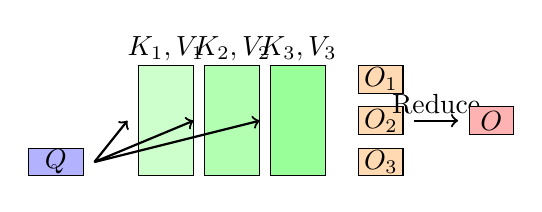
\begin{tikzpicture}[scale=0.7]
    % Q
    \draw[fill=blue!30] (0, 0) rectangle (1, 0.5);
    \node at (0.5, 0.25) {$Q$};

    % KV splits
    \draw[fill=green!20] (2, 0) rectangle (3, 2);
    \draw[fill=green!30] (3.2, 0) rectangle (4.2, 2);
    \draw[fill=green!40] (4.4, 0) rectangle (5.4, 2);
    \node at (2.5, 2.3) {$K_1, V_1$};
    \node at (3.7, 2.3) {$K_2, V_2$};
    \node at (4.9, 2.3) {$K_3, V_3$};

    % Parallel arrows
    \draw[->, thick] (1.2, 0.25) -- (1.8, 1);
    \draw[->, thick] (1.2, 0.25) -- (3, 1);
    \draw[->, thick] (1.2, 0.25) -- (4.2, 1);

    % Partial outputs
    \draw[fill=orange!30] (6, 1.5) rectangle (6.8, 2);
    \draw[fill=orange!30] (6, 0.75) rectangle (6.8, 1.25);
    \draw[fill=orange!30] (6, 0) rectangle (6.8, 0.5);
    \node at (6.4, 1.75) {$O_1$};
    \node at (6.4, 1) {$O_2$};
    \node at (6.4, 0.25) {$O_3$};

    % Reduce
    \draw[->, thick] (7, 1) -- (7.8, 1);
    \node at (7.4, 1.3) {Reduce};

    % Final output
    \draw[fill=red!30] (8, 0.75) rectangle (8.8, 1.25);
    \node at (8.4, 1) {$O$};
\end{tikzpicture}
\caption{Flash Decoding:KV序列并行 + Reduction}
\label{fig:flash_decoding}
\end{figure}

\subsubsection{性能提升}

\begin{itemize}
    \item 长序列解码加速高达\textbf{8倍}
    \item 在CodeLLaMa-34B上,注意力操作比FlashAttention快\textbf{50倍}
    \item 序列长度从512增加到64K,生成速度几乎不变
\end{itemize}

\subsection{FlashDecoding++}

FlashDecoding++~\citep{hong2024flashdecodingpp}进一步优化,在MLSys 2024发表。

\subsubsection{异步Softmax}

Flash Decoding的Reduction步骤需要同步等待所有部分结果。FlashDecoding++引入\textbf{Unified Max Value}:
\begin{itemize}
    \item 预估一个全局最大值$m_{unified}$(基于统计或启发式)
    \item 所有块使用相同的$m_{unified}$,无需同步
    \item 细粒度流水线,Prefill加速1.05$\times$,Decoding加速1.14$\times$
\end{itemize}

\subsubsection{Flat GEMM优化}

推理时的GEMM形状是``扁平''的($1 \times N$),标准实现效率低:
\begin{itemize}
    \item cuBLAS/CUTLASS对这种形状有高达50\%的性能损失
    \item FlashDecoding++使用Double Buffering和针对性优化
    \item Flat GEMM加速高达52\%
\end{itemize}

\subsubsection{启发式数据流}

根据输入形状动态选择最优数据流:
\begin{itemize}
    \item 不同序列长度、batch size有不同瓶颈
    \item 启发式选择避免静态数据流的50\%性能损失
\end{itemize}

\begin{table}[htbp]
\centering
\caption{Flash Decoding系列性能对比}
\label{tab:flash_decoding}
\begin{tabular}{lcc}
\toprule
方法 & 相对HuggingFace & 相对SOTA引擎 \\
\midrule
FlashAttention(推理) & 基线 & - \\
Flash Decoding & 8$\times$(长序列) & - \\
FlashDecoding++ & 4.86$\times$ & 1.37$\times$ \\
\bottomrule
\end{tabular}
\end{table}

\subsection{FlashAttention的工程影响}

FlashAttention已成为现代LLM训练和推理的\textbf{标配}:
\begin{itemize}
    \item \textbf{PyTorch 2.0+}:内置\texttt{scaled\_dot\_product\_attention}使用FlashAttention
    \item \textbf{vLLM、TensorRT-LLM}:推理引擎默认使用
    \item \textbf{所有主流LLM}:GPT-4、Claude、LLaMA、DeepSeek等都使用FlashAttention
\end{itemize}

\paragraph{上下文长度革命}
FlashAttention将实用上下文长度从2-4K提升到128K+:
\begin{itemize}
    \item 内存从$O(N^2)$降到$O(N)$
    \item 64K序列在标准注意力下需要16GB显存,FlashAttention只需约1GB
\end{itemize}

\begin{remark}[何时使用FlashAttention]
FlashAttention在以下场景收益最大:
\begin{itemize}
    \item \textbf{长序列}:序列长度$> 512$
    \item \textbf{大batch}:充分利用GPU并行
    \item \textbf{训练}:内存节省允许更大batch
\end{itemize}

短序列、小模型场景下,标准注意力可能更快(减少kernel launch开销)。
\end{remark}

\subsection{FlexAttention:可编程的FlashAttention}

FlexAttention是PyTorch 2.5引入的新API,提供FlashAttention的灵活编程接口。

\paragraph{动机}
FlashAttention虽然高效,但每种注意力变体(Causal、ALiBi、Sliding Window等)都需要专门实现。研究者想试验新变体时,往往需要手写Triton kernel。FlexAttention通过\texttt{torch.compile}自动生成高效kernel,将开发时间从数周缩短到数分钟。

\paragraph{核心API}
FlexAttention提供两个函数式接口:
\begin{itemize}
    \item \textbf{score\_mod}:修改$QK^\top$后的分数矩阵(如添加位置偏置)
    \item \textbf{mask\_mod}:定义mask模式(返回True的位置参与计算)
\end{itemize}

\begin{lstlisting}
from torch.nn.attention.flex_attention import flex_attention, create_block_mask

# Causal mask
def causal(b, h, q_idx, kv_idx):
    return q_idx >= kv_idx

# ALiBi位置编码
def alibi(score, b, h, q_idx, kv_idx):
    return score + (q_idx - kv_idx) * slope[h]

# 使用
block_mask = create_block_mask(causal, B, H, Q_LEN, KV_LEN)
out = flex_attention(q, k, v, score_mod=alibi, block_mask=block_mask)
\end{lstlisting}

\paragraph{性能}
FlexAttention达到FlashAttention-2约\textbf{85-90\%}的性能,但开发效率提升100倍。对于FlashAttention不原生支持的变体(如Document Masking),FlexAttention比标准SDPA快5-8倍。

\paragraph{适用场景}
\begin{itemize}
    \item 快速原型验证新的注意力变体
    \item 复杂mask模式(document masking、jagged tensors)
    \item 生产环境如果用标准变体,仍推荐直接使用FlashAttention
\end{itemize}

